%% ****** Start of file apsguide4-1.tex ****** %
%%
%%   This file is part of the APS files in the REVTeX 4.1 distribution.
%%   Version 4.1r of REVTeX, August 2010.
%%
%%   Copyright (c) 2009, 2010 The American Physical Society.
%%
%%   See the REVTeX 4.1 README file for restrictions and more information.
%%
\documentclass[twocolumn,secnumarabic,amssymb, nobibnotes, aps, prd]{revtex4-1}
%\usepackage{acrofont}%NOTE: Comment out this line for the release version!
\newcommand{\revtex}{REV\TeX\ }
\newcommand{\classoption}[1]{\texttt{#1}}
\newcommand{\macro}[1]{\texttt{\textbackslash#1}}
\newcommand{\m}[1]{\macro{#1}}
\newcommand{\env}[1]{\texttt{#1}}
\setlength{\textheight}{9.5in}



\usepackage{color}
\usepackage[latin9]{inputenc}
\usepackage{mathrsfs,amsmath}
\usepackage{graphicx}%
\usepackage{float}
\usepackage{amsfonts}%
\usepackage[titletoc]{appendix}
\usepackage{amssymb}
\usepackage{braket}
\usepackage{bm}

\newcommand{\mb}[1]{\bm{#1}}
\usepackage[T1]{fontenc}



\def\Nabla{\bm{\nabla}}
\def\bm{\mathbf}
\def\curl{\Nabla\times}
\def\div{\Nabla\cdot}
\def\lap{\Delta}
\def\vlap{\Delta}
\def\x{\hat{e}_{x}}
\def\y{\hat{e}_{y}}
\def\z{\hat{e}_{z}}
\def\p{\partial}
\def\h{\hat}
\DeclareMathOperator{\Tr}{Tr}

\bibliographystyle{ieeetr}
\begin{document}

\title{Spectral and Temporal Hole Burning in Quantum Cascade Lasers with Strong Injector Anticrossing}%

\author{Petar Tzenov}%
\email{petar.tzenov@tum.de}
\affiliation{Institute for Nanoelectronics, Technical University of Munich, D-80333 Munich, Germany}
\date{June 8, 2016}%
\maketitle
\tableofcontents

\section{Introduction}
We will theoretically and numerically demonstrate the formation of a temporal grating in quantum cascade lasers due to strong injector anticrossing between subbands spanning an intermodule barrier. 

Let us consider a simple toy configuration, consisting of two quantum wells per period, and let us take two periods, separated by a thick tunneling barrier, see Fig. \ref{fig:threelvl}. Let us assume that 
at design bias, the tight-binding basis ground state, $\Ket{s}$, of the left well aligns with  the first excited state $\Ket{e}$ of the right well, with some small detuning energy $E_{s}-E_{e} = \hbar \epsilon$. On the other hand, let us assume that the energetic difference between the state $\Ket{e}$ and the ground state of the right well, $\Ket{g}$ is given as $E_{e}- E_{g} = \hbar\omega_0 $, which can be assumed to lie in the terahertz (THz) range. 
 \begin{figure}[h!]
 	\begin{center}
 		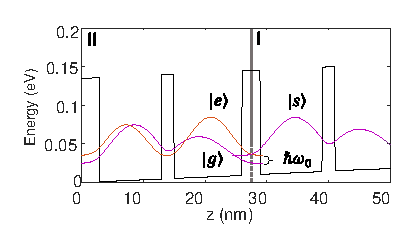
\includegraphics[scale=1.0]{threelvlSystem.eps}
 		\caption{Schematic illustration of a 3 level QCL system with a strong "injector" $\leftrightarrow$ "upper laser level" coupling. State $\ket{s}$ couples to $\ket{e}$ (the upper laser level) via resonant tunneling, whereas $\ket{e}$ couples to the ground state $\ket{g}$ radiatively. The wave functions have been calculated within the tight-binding basis with our Schr�dinger-Poisson solver.  }\label{fig:threelvl}
 	\end{center}	
 \end{figure}
In the tight binding basis, the alignment between the left ground state and the right excited state causes an energetic splitting, characterized by the anticrossing energy $\hbar\Omega_{se}$. Finally assuming an incident terahertz electromagnetic field $E(x,t)$, oscillating with central frequency $\omega_c$, which is near resonance with the $\Ket{e}\leftrightarrow\Ket{g}$ transition, i.e. $\omega_0 \approx \omega_c$, we can write down the tight-binding Hamiltonian of the system within the electric dipole approximation as

\begin{align}
	\label{eq:hamiltonian-operatorform}
	\h{H} &= \hbar(\epsilon + \omega_0) \h\sigma_{s,s} +\hbar\omega_0\h\sigma_{e,e}  \nonumber \\ 
	& +(\hbar\Omega_{se}\h\sigma_{s,e} +q_0d_{eg}E\h\sigma_{e,g}+h.c.),
\end{align}
where we have set the zero energy as the ground state energy, $d_{eg}=\Bra{e}\h z \Ket{g}$  denotes the dipole moment matrix element, $\h z$ is the position operator along the growth direction $z$, $q_0$ is the elementary charge and finally $\h \sigma_{i,j}$ are the atomic projection operators. Taking the states $\Ket{s},\Ket{e}$ and $\Ket{g}$ as a complete orthonormal basis,  the Hamiltonian in Eq. (\ref{eq:hamiltonian-operatorform}) can be cast into matrix form as

\begin{align}
\label{eq:hamiltonian-matrixform}
H &= \begin{pmatrix}
\hbar(\epsilon + \omega_0) & \hbar \Omega_{se} & 0 \\ 
\hbar \Omega_{se} & \hbar\omega_0 & q_0d_{eg}E \\
0 & q_0d_{eg}E & 0
\end{pmatrix}.
\end{align}

To model the light-matter interaction dynamics we will employ a density matrix approach to describe the statistical behaviour of the atomic ensemble in our system, coupled to the classical Maxwell's equations via a polarization term. 

The time evolution of the density matrix is governed by the von Neumann equation
\begin{equation}
\frac{d \rho}{dt} = \frac{i}{\hbar} [\rho,H],
\end{equation}
where $[\cdot,\cdot]$ is the matrix commutator. Additionally there need to be included phenomenological scattering terms to model non-radiative incoherent scattering processes between different subbands of our system. The final form of the equation of motion, which we will consider, is therefore
\begin{equation}
\frac{d \rho}{dt} = \frac{i}{\hbar} [\rho,H] + coll,  
\end{equation}
where $coll$ denotes all collision terms (include in detail later). Including space dependence and employing the slowly varying envelope and rotating wave approximation we get the following system of equations (standard Maxwell-Bloch equations system for a ring cavity configuration, i.e. no spatial hole burning is taken into accoutn)
\begin{center}
\begin{widetext}
\begin{subequations}
	\label{eq:threelevelmodel}
	\begin{align}
	 \frac{n}{c}\partial_t f &+ \partial_{x}f= -i\frac{N \Gamma q_0d_{eg} k_c}{\epsilon_0 n^2} \eta_{eg} - \frac{l_0}{2} f \label{eq:rtwave} \\
		\frac{d \rho_{ss}}{d t} 	&= i\Omega_{se} (\rho_{se} - \rho_{es})+ \Gamma_{es}\rho_{ee} + \Gamma_{gs}\rho_{gg}  -\Gamma_s\rho_{ss} \\
		\frac{d \rho_{ee}}{d t}	& = i\Omega_{se} (\rho_{es} - \rho_{se}) + i\frac{q_0d_{eg}}{2\hbar} \big (f^*\eta_{eg}- c.c. \big ) 
		 +\Gamma_{se}\rho_{ss} + \Gamma_{ge}\rho_{gg} - \Gamma_e \rho_{ee},  \\
		\frac{d \rho_{gg}}{d t}  &= -i\frac{q_0d_{eg}}{2\hbar} \big (f^*\eta_{eg} - c.c. \big )  + \Gamma_{sg}\rho_{ss}  +  \Gamma_{eg}\rho_{ee} - \Gamma_{gg}\rho_{gg} , \\
		\frac{d \rho_{se}}{d t}  &= -i\epsilon\rho_{se} +i \Omega_{se}(\rho_{ss} - \rho_{ee}) +i\frac{q_0d_{eg}}{2 \hbar}f^*\eta_{sg}- \Gamma_{\parallel se} \rho_{se},  \\
		\frac{d \eta_{eg}}{d t}   &= i(\omega_c - \omega_0)\eta_{eg} + i \frac{q_0d_{eg}}{2\hbar}f(\rho_{ee}-\rho_{gg})  -i\Omega_{se}\eta_{sg} - \Gamma_{\parallel eg}\eta_{eg}, \\
		\frac{d \eta_{sg}}{d t} &= i(\omega_c - \omega_0-\epsilon)\eta_{sg} +i \frac{q_0d_{eg}}{2\hbar}f\rho_{se} - i\Omega_{se}\eta_{eg} - \Gamma_{\parallel sg}\eta_{sg}.
	\end{align}
\end{subequations}
\end{widetext}
\end{center}
Above, we have made the following assumptions 
\begin{align}
E(x,t) &= \frac{1}{2} (f(x,t) e^{i(k_cx-\omega_c t)}+c.c.),\\
\rho_{eg} &= \eta_{eg}e^{i(k_cx-\omega_c t)}, \\
\rho_{sg} &= \eta_{sg}e^{i(k_cx-\omega_c t)}, 
\end{align}
and, within the framework of the rotating wave approximation, neglected terms, oscillating faster than $e^{\pm i\omega_c t}$. Also, $\Gamma_{ij} $ denote the scattering rates from state $\ket{i}$ to state $\ket{j}$, $\Gamma_k = \sum_{j}\Gamma_{kj}$ is the total out-scattering rate from level $\ket{k}$ and $\Gamma_{\parallel ij} = \frac{1}{2}(\Gamma_{i} + \Gamma_j) + \Gamma_{i,j}^*$ with $\Gamma_{i,j}^*$ the pure dephasing rate for the transition $i\rightarrow j$ (which, in principle, we can calculate with our Monte-Carlo software). 


\section{Spectral hole burning due to strong injector anticrossing}
 
The introduction of the coupling energy $\hbar \Omega_{se}$ into the Hamiltonian of the system contributes to a splitting of the optical spectra into a high and a low frequency lobes. This is due to the fact that the extended system's Hamiltonian is non-diagonal in the tight binding basis. The new eigenstates, which diagonalize the Hamiltonian in Eq. (\ref{eq:hamiltonian-matrixform}), are the so called dressed states \cite{dupont2010simplified} and are obtained from $\Ket{s}$ and $\Ket{e}$ via the unitary transformation
 \begin{align}
 \label{eq:dressedstates}
 \Ket{+} &= \cos\theta \Ket{s} - \sin\theta \Ket{e}, \nonumber \\
 \Ket{-} &= \sin\theta \Ket{s} + \cos\theta \Ket{e}.
 \end{align}
 The corresponding energies are given by $E_\pm =\hbar(\omega_0 +\frac{\epsilon}{2}) \pm \hbar\sqrt{\epsilon^2+4\Omega_{se}^2}$, where the coefficients are computed from  
 $
 \tan \theta = -2\Omega_{se}/(\epsilon+\sqrt{\epsilon^2+4\Omega_{se}^2}).
 $
 \begin{figure}[h!]
 	\begin{center}
 		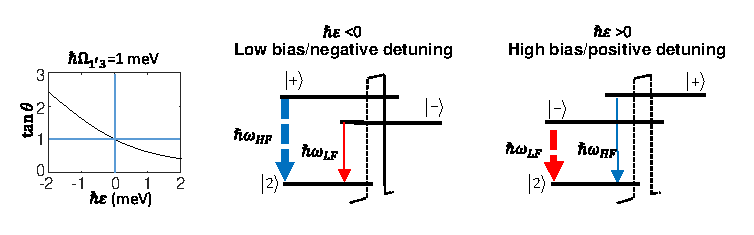
\includegraphics[scale=0.75]{BIASDETUNING.eps}
 		\caption{ Schematic illustration of the dependence of the high and low frequency transitions on bias. (Left column) Plot of $\tan\theta$ as a function of detuning from resonance. (Middle and right columns) The relative oscillator strengths (thicker arrow represents higher value) when the laser is biased below and above resonance, respectively. } \label{fig:detuning}
 	\end{center}	
 \end{figure}
  
 Here we remind the reader that the detuning from $\Ket {s}\leftrightarrow\Ket{e}$ resonance is given by $E_{s} - E_{e} = \hbar\epsilon$. We can compute the ratio of the dipole matrix elements for the $\Ket{+}\leftrightarrow\Ket{g}$ and $\Ket{-}\leftrightarrow\Ket{g}$ transitions, which will determine the relative strength between the high and low frequency lobes of the gain. Thus
 \begin{align}
 \label{eq:dresseddipoles}
 \left |\frac{\Bra{+}\hat{\mu}\Ket{g}}{\Bra{-}\hat{\mu}\Ket{g}}\right | \approx |\tan\theta| =  \frac{2|\Omega_{se}|}{|\epsilon+\sqrt{\epsilon^2+4\Omega_{se}^2}|},
 \end{align}
 where we assume that $\mu_{sg} \approx 0$.
 We now can easily see that at high biases, i.e. positive detunings $\epsilon >0$, $|\tan\theta|<1$ and thus the low frequency transition will have higher probability. On the other hand, for $\epsilon < 0 $ we get that $|\tan\theta| >1$ which will lead to lasing predominantly in the high frequency regime. This behaviour above and below resonant bias is schematically illustrated in Fig. \ref{fig:detuning}, where $\hbar\omega_{LF} $ and $\hbar\omega_{HF}$ denote the energy of the low and high frequency transition respectively and the anticrossing energy is set at $\hbar \Omega_{1'3} = 1$ meV.  
 
 
\section{Temporal hole burning due to strong injector anticrossing}
Let us further investigate the effect of the spectral splitting onto the temporal dynamics of our system by taking the following, additional ansatz for the envelope $f(x,t)$ and accordingly the coherences
\begin{subequations}
\begin{align}
	\label{eq:splittingAnsatz}
	f &= f^{(\delta)}e^{i(\delta k x  - \delta\omega t)} + f^{(-\delta)}e^{-i(\delta kx-\delta\omega t)}, \\
	\eta_{eg} &= \eta_{eg}^{(\delta)}e^{i(\delta k x  - \delta\omega t)} + \eta_{eg}^{(-\delta)}e^{-i(\delta kx-\delta\omega t)}, \\
	\eta_{sg} &= \eta_{sg}^{(\delta)}e^{i(\delta k x  - \delta\omega t)} + \eta_{sg}^{(-\delta)}e^{-i(\delta kx-\delta\omega t)},
\end{align}
\end{subequations}
where $\delta\omega \approx \Omega_{se}$  is around \emph{half} the anticrossing energy due to the tunneling transition. Thus we have separated the electric field envelope $f$ and the coherences $\eta_{sg}$, $\eta_{eg}$ into components oscillating with frequencies around the high and low frequency spectral components of the signal, respectively. We use the above ansatz to evaluate the products $f^*\eta_{sg}$ and $f^*\eta_{eg}$ in Eq. (\ref{eq:threelevelmodel}) at $x=0$ (for convenience). Using the index $j$ as a place holder for $eg$ and  $sg$ we obtain
\begin{widetext}
\begin{align}
	\label{eq:feta-product}
	f^{*}\eta_{j} &= ((f^{(\delta)})^*e^{  i\delta\omega t} + (f^{(-\delta)})^*e^{-i\delta\omega t})(\eta_{j}^{(\delta)}e^{ - i\delta\omega t} + \eta_{j}^{(-\delta)}e^{+i\delta\omega t}) \nonumber \\
			&= \big[ (f^{(\delta)})^*\eta_{j}^{(\delta)} +(f^{(-\delta)})^*\eta_{j}^{(-\delta)} + (f^{(\delta)})^*\eta_{j}^{(-\delta)}e^{2i\delta\omega t} + (f^{(-\delta)})^*\eta_{j}^{(\delta)}e^{-2i\delta\omega t}\big ].
\end{align} 
\end{widetext}
We can reconcile this result with Eq. (\ref{eq:threelevelmodel}) if we extend it with the following ansatz for the  population densities and the $\rho_{se}$ coherence term 
\begin{align}
	\rho_{jj} &= \rho_{jj}^{DC}+\rho_{jj}^{+}e^{2i(\delta k x-\delta \omega t)} + \rho_{jj}^{-}e^{-2i(\delta k x-\delta \omega t)}, \\
	\rho_{se} &= \rho_{se}^{DC}+\rho_{se}^{+}e^{2i(\delta k x-\delta \omega t)} + \rho_{se}^{-}e^{-2i(\delta k x-\delta \omega t)},
\end{align}
where $j \in \{s,e,g\}$, $\rho_{jj}^{-} = (\rho_{jj}^{(+)})^*$ and $\rho_{se}^{-} = (\rho_{es}^{+})^*$ due to the Hermitian property of the density matrix. Then, we can derive the evolution equations for $\rho_{jj}^{DC},\rho_{jj}^{\pm}$ and $\rho_{se}$ as follows (setting again x =0 for convenience)

\begin{widetext}
	\begin{align}
	\label{eq:temporal-hole-ss}
	\frac{d\rho_{ss}^{DC}}{dt} &= i\Omega_{se}(\rho_{se}^{DC}-\rho_{es}^{DC}) +  \Gamma_{es}\rho_{ee}^{DC} + \Gamma_{gs}\rho_{gg}^{DC}  -\Gamma_s\rho_{ss}^{DC}, \\
	\frac{d\rho_{ss}^{+}}{dt} &= 2i\delta\omega\rho_{ss}^{+} + i\Omega_{se}(\rho_{se}^{+}-\rho_{es}^{+}) +  \Gamma_{es}\rho_{ee}^{+} + \Gamma_{gs}\rho_{gg}^{+}  -\Gamma_s\rho_{ss}^{+},
	\end{align} 
\end{widetext}

\begin{widetext}
	\begin{align}
	\label{eq:temporal-hole-ee}
	\frac{d\rho_{ee}^{DC}}{dt} &= i\Omega_{se}(\rho_{es}^{DC}-\rho_{es}^{DC}) + i\frac{q_0d_{eg}}{2\hbar} \left [ ( f^{(\delta)})^*\eta_{eg}^{(\delta)} +(f^{(-\delta)})^*\eta_{eg}^{(-\delta)} -c.c.\right]
	+\Gamma_{se}\rho_{ss}^{DC} + \Gamma_{ge}\rho_{gg}^{DC} - \Gamma_e \rho_{ee}^{DC}, \\
	\frac{d\rho_{ee}^{+}}{dt} &= 2i\delta\omega\rho_{ee}^{+}  + i\Omega_{se}(\rho_{es}^{+}-\rho_{es}^{+}) + i\frac{q_0d_{eg}}{2\hbar} \left [ (f^{(\delta)})^*\eta_{eg}^{(-\delta)} -f^{(-\delta)}(\eta_{eg}^{(\delta)})^*\right]
	+\Gamma_{se}\rho_{ss}^{+} + \Gamma_{ge}\rho_{gg}^{+} - \Gamma_e \rho_{ee}^{+}, \\
	\frac{d\rho_{gg}^{DC}}{dt} &= -i\frac{q_0d_{eg}}{2\hbar} \left [ ( f^{(\delta)})^*\eta_{eg}^{(\delta)} +(f^{(-\delta)})^*\eta_{eg}^{(-\delta)} -c.c.\right]
	+\Gamma_{sg}\rho_{ss}^{DC} + \Gamma_{eg}\rho_{ee}^{DC} - \Gamma_g \rho_{gg}^{DC}, \\
	\frac{d\rho_{gg}^{+}}{dt} &= 2i\delta\omega\rho_{gg}^{+} - i\frac{q_0d_{eg}}{2\hbar} \left [  (f^{(\delta)})^*\eta_{eg}^{(-\delta)} -f^{(-\delta)}(\eta_{eg}^{(\delta)})^*\right]
	+\Gamma_{sg}\rho_{ss}^{+} + \Gamma_{eg}\rho_{ee}^{+} - \Gamma_g \rho_{gg}^{+},
\end{align}

\begin{align}	
	\frac{d \rho_{se}^{DC}}{d t}  &= -i\epsilon\rho_{se}^{DC} +i \Omega_{se}(\rho_{ss}^{DC} - \rho_{ee}^{DC}) +i\frac{q_0d_{eg}}{2 \hbar}((f^{(\delta)})^*\eta_{sg}^{(\delta)} +(f^{(-\delta)})^*\eta_{sg}^{(-\delta)})- \Gamma_{\parallel se} \rho_{se}^{DC},  \\
	\frac{d \rho_{se}^{+}}{d t}  &= i(2\delta\omega-\epsilon\rho_{se}^{DC}) +i \Omega_{se}(\rho_{ss}^{+} - \rho_{ee}^{+}) +i\frac{q_0d_{eg}}{2 \hbar}( (f^{(-\delta)})^*\eta_{sg}^{(\delta)} )- \Gamma_{\parallel se} \rho_{se}^{+},\\
	\frac{d \rho_{se}^{-}}{d t}  &= -i(2\delta\omega+\epsilon\rho_{se}^{DC}) +i \Omega_{se}(\rho_{ss}^{-} - \rho_{ee}^{-}) +i\frac{q_0d_{eg}}{2 \hbar}( (f^{(\delta)})^*\eta_{sg}^{(-\delta)} )- \Gamma_{\parallel se} \rho_{se}^{-},  \\
	\frac{d \eta_{eg}^{(\pm\delta)}}{d t} &= i(\omega_c-\omega_0\pm \delta\omega)\eta_{eg}^{(\pm\delta)}
	+i\frac{q_0d_{eg}}{2\hbar} ( f^{(\pm\delta)}(\rho_{ee}-\rho_{gg})^{DC} + f^{(\mp \delta)} (\rho_{ee}-\rho_{gg})^{\pm})-i\Omega_{se}\eta_{sg}^{(\pm\delta)}- \Gamma_{\parallel eg}\eta_{eg}^{(\pm\delta)}, \label{eq:etase-temphole} \\
	\frac{d \eta_{sg}^{(\pm\delta)}}{d t} &= i(\omega_c-\omega_0-\epsilon \pm \delta\omega)\eta_{sg}^{(\pm\delta)}+i\frac{q_0d_{eg}}{2\hbar} ( f^{(\pm\delta)}\rho_{se}^{DC} + f^{(\mp \delta)} \rho_{se}^{\pm})-i\Omega_{se}\eta_{eg}^{(\pm\delta)}- \Gamma_{\parallel eg}\eta_{sg}^{(\pm\delta)}. \label{eq:etasg-temphole}
	\end{align} 
\end{widetext}

It is worthwhile to note that in the above derivation of Eq. (\ref{eq:etase-temphole},\ref{eq:etasg-temphole}) we have neglected terms proportional to $e^{\pm 3\delta \omega t}$. Finally, we can expand the wave propagation equations within our familiar ansatz and we see that the high and low frequency lobes satisfy
\begin{align}
 \frac{n}{c}\partial_t f^{(\pm \delta)} + \partial_{x}f^{(\pm \delta)}&= -i\frac{N \Gamma q_0d_{eg} k_c}{\epsilon_0 n^2} \eta_{eg}^{(\pm \delta)} \nonumber \\ 
			&- \left[\frac{l_0}{2}  \pm i (\frac{n\delta\omega}{c}-\delta k)\right] f^{(\pm \delta)}\label{eq:rtwave-temphole},
\end{align}
which includes both linear losses, via a constant term $l_0$, as well as chromatic dispersion, due to modification of the real part of the refractive index via the term  $\pm i (\frac{n\delta\omega}{c}-\delta k)$. Notice also that the above system is very familiar. It is almost identical to the spatial hole burning effect \cite{wang2007coherent}, however this time the grating is in time not space. 

\section{Simulation results}
UNDER DEVELOPMENT

\bibliography{literature.bib}
\end{document}

